% THIS IS A LATEX TEMPLATE FILE FOR PAPERS INCLUDED IN THE
% *Anthology of Computers and the Humanities*. ADD THE OPTION
% 'final' WHEN CREATING THE FINAL VERSION OF THE PAPER. 
% DO NOT change the documentclass
%\documentclass[final]{anthology-ch} % for the final version
\documentclass[final]{anthology-ch}         % for the submission

% LOAD LaTeX PACKAGES
\usepackage{booktabs}
\usepackage{graphicx}
\usepackage{listings}
\usepackage{xcolor}

\lstset{
  basicstyle=\ttfamily\footnotesize,
  breaklines=true,
  breakatwhitespace=true,
  columns=fullflexible,
  frame=single,
  backgroundcolor=\color{gray!10},
  captionpos=b,
  keepspaces=true
}


\title{The Illustrated Page: Analyzing Illustrations of Historical Children’s Books Using Citizen Science}

% A Citizen-Science Dataset of Historical Children’s Book Images

% Illustrating the Past: Analyzing Historical Children’s Book Illustrations at Scale

% Picturing Stories: A large scale data set of annotated historical children's book illustrations derived using citizen science


% AUTHOR AND AFFILIATION INFORMATION
% For each author, include a new call to the \author command, with
% the numbers in brackets indicating the associated affiliations 
% (next section) and ORCID-ID for each author.  
\author[1]{Andrew Piper}[
  orcid=0000-0001-9663-5999
]

\author[2]{Jiaming Jiang}[
  orcid=0009-0001-9699-7698
]

% While we encourage including ORCID-IDs for all authors, you can
% include authors that do not have one by definining an empty ID.
\author[3]{Robert Budac}[
  orcid=0009-0003-5901-1919
]

% There should be one call to \affiliation for each affiliation of
% the authors. Multiple affiliations can be given to each author
% and an affiliation can be given to multiple authors. 
\affiliation{1}{Department of Languages, Literatures, and Cultures, McGill University, Montreal, Canada}
\affiliation{2}{College of Humanities, EPFL, Lausanne, Switzerland}
\affiliation{3}{Digital Humanities, University of Alberta, Edmonton, Canada}

% KEYWORDS
% Provide one or more keywords or key phrases seperated by commas
% using the following command
\keywords{children's literature, illustrated books, history of print, image understanding, citizen science, distant viewing}

% METADATA FOR THE PUBLICATION
% This will be filled in when the document is published; the values can
% be kept as their defaults when the file is submitted
\pubyear{2025}
\pubvolume{3}
\pagestart{279}
\pageend{293}
\conferencename{Computational Humanities Research 2025}
\conferenceeditors{Taylor Arnold, Margherita Fantoli, and Ruben Ros}
\doi{10.63744/XVr0QDckSvkj}  
\paperorder{20}


\addbibresource{bibliography.bib}

%%%%%%%%%%%%%%%%%%%%%%%%%%%%%%%%%%%%%%%%%%%%%%%%%%%%%%%%%%%%%%%%%%%%%%%%%%%
% HERE IS THE START OF THE TEXT
\begin{document}

\maketitle

\begin{abstract}
This paper presents the first large-scale, systematic study of historical children’s book illustrations through a combination of citizen science and computational analysis. Using a corpus of 27,901 digitized illustrations from 2,827 books from the Internet Archive’s Children’s Library, we developed a structured annotation workflow deployed on Zooniverse to collect over 400,000 annotations from 902 volunteers. Tasks included identifying depicted characters, objects, settings, and emotional tone. We assess inter-annotator reliability across task types and derive consensus labels to explore three central questions: who and what is most commonly visualized, which entities co-occur, and how visual depictions change over time. Findings reveal dominant portrayals of patriarchal figures and animals, the centrality of nature, and gendered patterns in emotional framing. Temporal analysis shows a surprising visual stability over 140 years. This work demonstrates the value of human-in-the-loop annotation for visual cultural heritage and provides a new resource for studying the visual language of childhood in print. 
\end{abstract}

\section{Introduction} 

Illustrated children’s books offer a rich archive for understanding cultural history, combining visual and textual modes of storytelling that reflect societal values across time. Scholars have long emphasized that picture books are complex narrative artifacts in which words and images interact to produce meaning \cite{nodelman1988words, nikolajeva2002rhetoric}. This multimodal structure makes them powerful instruments of cultural transmission, encoding assumptions about childhood, gender, identity, morality, and emotion within their language and visual design \cite{kummerling2023picturebooks, grenby2009cambridge}. Historical studies have traced how these books foreground ideological currents and pedagogical aims, while psychological research underscores their formative role in early cognitive and emotional development \cite{kummerling2017picturebooks, montag2015words, wang2025picture}. Yet despite this longstanding interdisciplinary recognition, large-scale analysis of historical children’s book illustrations remains limited especially with respect to their visual content.

Illustrations in children’s books have long been read not merely as decorative accompaniments to text, but as cultural documents that encode shifting ideas of childhood and social order. Historians of childhood have shown how visual culture participates in defining what it means to be a child, often reinforcing classed, gendered, and racialized norms about innocence, obedience, play, and agency \cite{aries1962childhood, jenkins1998children,roethler1998reading,cunningham2020children, gittins2009historical}. Studies of children’s book illustration similarly emphasize the visual construction of gender roles, family relations, and moral conduct, revealing how images work pedagogically to shape expectations of behavior and identity \cite{brown2008capturing, roethler1998reading, crain2016reading}. At the same time, feminist and queer studies scholarship has highlighted the ways illustrations reproduce or contest cultural hierarchies, offering insights into how visual storytelling both reflects and regulates broader social imaginaries \cite{kincaid2013producing, pifer2000demon, thiel2013fantasy}.

To support deeper computational research into the representation of childhood, this paper introduces a new dataset of ca. 28,000 annotated children’s book illustrations created through an on-going citizen science project called ``Picturing Children's Stories.''\footnote{\url{https://www.zooniverse.org/projects/citizenreaders/picturing-childrens-stories}} The project aims to enlist the public to help build more transparent, human-centered AI models for understanding human storytelling. The dataset is derived from the Internet Archive's Children's Library, which consists of 2,827 digitized books published between the years 1728 and 1932.\footnote{\url{https://archive.org/details/iacl}} The first phase of annotations focuses on identifying core visual features associated with character age, gender, setting, the physical environment (objects and structures), and an assessment of emotional intensity to identify the degree of agency and activation connected to different character types and settings. Doing so allows us initial insights into the changing presence over time of different character types, social relationships, physical environments, and the emotional associations surrounding these interactions. The full dataset can be found here.\footnote{\url{https://doi.org/10.5683/SP3/KTSY9B}}

\section{Background}

Recent advances in multimodal large language models (MLLMs) have opened new possibilities for the automated analysis of cultural heritage images. To support this work, researchers have developed specialized datasets such as SemArt \cite{garcia2018read}, ArtPedia \cite{stefanini2019artpedia}, ArtCap \cite{lu2022artcap}, and DEArt \cite{reshetnikov2022deart}, which pair artworks with expert descriptions, iconographic labels, or object annotations. These resources have enabled the training of captioning models that incorporate art-historical knowledge \cite{bai2021explain} and the evaluation of zero-shot classification and metadata prediction by general-purpose LLMs \cite{tojima2025zero, rei2023multimodal}. Arnold and Tilton \cite{arnold2024explainable} propose a general framework for using MLLMs to generate textual captions and embedding-based similarity scores for large image corpora. Their approach supports explainable recommendations and cluster-based exploration of visual heritage collections, demonstrating how automated captioning can enhance searchability and interpretability without the need for pre-annotated metadata. Further work has also explored the interpretibity of historical newspaper illustrations \cite{fyfe2018image}, photographs \cite{arnold2024color, maksimova2024viability}, maps \cite{mahowald2024clip}, as well as graphical aspects of scientific publishing \cite{piper2020page, lang2023alchemy}, providing a broad range of approaches to studying visual cultural heritage materials. 

Compared to canonical artworks or photographs, historical book illustrations present distinct challenges for image understanding tasks \cite{mak2011page, berne2024design}. Unlike paintings, which are self-contained visual artifacts, or photographs which are more closely aligned with contemporary training data, book illustrations are embedded within larger narrative or instructional texts, such that their meaning often relies on sparser visual representations. Many illustrations are also low-resolution, monochromatic, or stylistically constrained by period-specific reproduction methods such as woodcuts or engravings. Additionally, some are subject to conditions of historical decay such as ``foxing,'' where mold or oxidation commences prior to digitization, or quirks of historical production such as ``show-through,'' when ink from the opposite side of a page shows through, and ``off-setting,'' when ink from another page bleeds onto the back of the page. As a result, accurately interpreting these images requires models to recognize subtle, often noisy visual cues and historical iconography that may be underrepresented in modern training data or art historical data.

\section{Data}

\subsection{Overview} 

Illustrations were sourced from a collection of 2,827 digitized books available through the Internet Archive's Children's Library. Over 91\% of books included in the collection are English-language books, with the next most represented language being French at just under 5\%. Based on an analysis of available regional information, we estimate that books originate equally from Britain and North America. To extract candidate images for annotation, we used PyMuPDF\footnote{https://github.com/pymupdf/PyMuPDF} to statistically analyze gray-scaled page images and identify illustration-containing pages. This resulted in 31,051 candidate page images. \autoref{fig:histogram} shows the distribution of publication dates of illustrations. 

To support the large-scale human annotation of page images, we developed a citizen science project using the platform Zooniverse.org. \autoref{fig:homepage} in the Appendix shows the project homepage. The project interface included a number of features to support the reliable classification of material: an ``About'' page to inform participants of the purpose of the research and how the data will be handled; a tutorial which guides participants through the task structure; pop-up help boxes that provide further examples/instructions; and finally talk pages where participants can pose questions to researchers, where we had a dedicated team of three moderators.  

Over a two-week period between May 20 and June 2, 2025, a total of 902 volunteers contributed a total of 457,756 annotations. Engagement was varied with 7.3\% of users completing only one annotated image, while the top 25\% of contributors accounted for 80\% of all annotation activity. In all, 27,901 illustrations were positively identified by a consensus of annotators (i.e. majority vote).

\begin{figure}[h!]
  \centering
  \includegraphics[width=0.6\linewidth]{figures/fig_Illustration_IA_histogram.png}
  \caption{Distribution of publication dates of illustrations in the Internet Archive Children's Library.}
  \label{fig:histogram}
\end{figure}

\subsection{Task Structure} 

\begin{figure}[h!]
  \centering
  \includegraphics[width=0.7\linewidth]{figures/Worklow_Images_Task_Example.jpg}
  \caption{Example screenshot of one stage of the task workflow.}
  \label{fig:task_example}
\end{figure}

Participants were presented with digitized pages from historical children’s books and asked to complete a structured sequence of annotation tasks based on the visual and textual content of each page (see \autoref{fig:task_example} for an example of the task interface). We required a retirement rate of three annotators per image. The workflow began with a screening question asking whether the page contained an illustration. We defined an illustration as: 

\begin{quote}
\textit{An illustration is a realistic image of a scene or person from a story. An illustration is NOT: decorative graphics, a logo, book stamp, or photograph.}
\end{quote}

\noindent Based on the majority agreement of annotators, we found that roughly 10\% (ca. 3,150) of all extracted images were labeled as non-illustrations according to our criteria. This is a valuable step in the workflow given that the distinction between visual elements that are and are not considered illustrations can be very subtle.

If the participant answered ``Yes'' to this question, they were then guided through a series of visual classification tasks concerning the illustration as shown in \autoref{tab:tasks}. These included identifying the age, gender, and species of characters (T1); whether the illustration was set indoors or outdoors (T2); the objects and structures depicted (T3); and the emotional intensity of the scene (T4). Each task was presented with an optional tutorial and contextual help, ensuring consistent interpretation across annotators. 

This workflow was designed to balance interpretive nuance with structured metadata collection to facilitate both future analysis and multi-modal large-language model training. Entity types and their co-occurrence can help us understand the overall visual presence of entities over time, depicted social structures, orientations towards the natural and built environment, along with the emotional association of these interactions. We chose to focus on ``emotional intensity'' (also known as ``arousal'' in the psychological literature) for two reasons. The first is this is a well-established concept in psychology \cite{russell1980circumplex} and computational text analysis \cite{mohammad2018obtaining}. Second, we found this emotional dimension the most relevant for contextualizing the emotional agency of characters, which can begin to give us insights into the ideological portrayal of entities in children's books.

\begin{table}[ht]
\centering
\begin{tabular}{p{.5cm} p{2cm} p{4cm} p{6cm}}
\toprule
\textbf{Task} & \textbf{Category} & \textbf{Question} & \textbf{Possible Answers} \\
\midrule
T0 & Illustration & Is there an illustration on this page? & \textit{Yes, No} \\
\hline
T1 & Characters & Who are the characters on the page? Check all that apply. & \textit{Man, Woman, Girl, Boy, Animal, Animate Object (e.g., a teddy bear or spoon who talks), Mythical / Imaginary Being, Other, None} \\
\hline
T2 & Setting & Where is the scene set? & \textit{Indoors, Outdoors, Both / Ambiguous} \\
\hline
T3 & Objects & What are the main objects in the scene? Check all that apply. & \textit{Nature (trees, flowers, lakes), Architecture (buildings, walls, furniture), Vehicles (cars, boats, planes), Toys, Reading and Art (books, musical instruments, paintings), Household items and tools (pots, pans, hammers, sticks), Other, None} \\
\hline
T4 & Intensity & How emotionally intense is this scene? What is the energy like? & \textit{1 - Very calm (still, contemplative, restful), 2 - Mildly calm, 3 - Neutral, 4 - Mildly intense, 5 - Very intense (frantic, tense, active)} \\
\bottomrule
\end{tabular}
\caption{Annotation task structure: order, categories, questions, and response options.}
\label{tab:tasks}
\end{table}

\subsection{Inter-Annotator Agreement}

To assess the reliability of the citizen-science annotations, we computed inter-annotator agreement separately for each task type. Tasks varied in structure: some required a single categorical response (T0, T2), others allowed for multiple selections (T1,T3), and one required ordinal judgments (T4). Table \ref{tab:iaa_summary} summarizes the different agreement measures across tasks.

For the single-answer tasks (T0, T2), we measured the percentage of majority versus full agreement as an intuitive baseline of how much disagreement there was. We did not use a traditional IAA measure such as Krippendorff’s alpha due to the sparsity of annotator coverage across items—most participants annotated only a small subset of the dataset—violating the assumptions of that metric. As we can see in \autoref{tab:iaa_summary}, agreement was high for both single-answer tasks, with 85\% full agreement on the presence of an illustration and 93\% full agreement on indoor/outdoor setting. The former is particularly surprising given the number of potential edge cases with decorative headpieces or borders.

For multi-answer tasks (T1 and T3), we calculated agreement using pairwise Jaccard similarity: the size of the intersection divided by the size of the union of label sets across annotators. Each item’s agreement score was computed as the mean Jaccard similarity across all annotator pairs. Results showed moderate to high consistency. For T1 (character types), the mean Jaccard similarity across items was 0.73 (median = 0.78), with 25\% of items showing perfect agreement (score = 1.0). For T3 (object types), the average was lower at 0.22 (median = 0.56), suggesting greater subjectivity and label diversity in this task.

To put these scores into context, we provide two illustrative scenarios involving hypothetical annotators assigning character labels and their attendant Jaccard agreement scores:

\begin{itemize}
  \item \textbf{Example 1: High Agreement}
  \begin{itemize}
    \item Annotator A: \{Man, Woman, Girl\}, Annotator B: \{Man, Woman, Girl, Boy\}
    \item Intersection: \{Man, Woman, Girl\} = 3, Union: \{Man, Woman, Girl, Boy\} = 4
    \item Jaccard similarity: \( \frac{3}{4} = 0.75 \)
  \end{itemize}

  \item \textbf{Example 2: Moderate Agreement}
  \begin{itemize}
    \item Annotator A: \{Man, Woman\}, Annotator B: \{Man, Woman, Girl, Boy\}
    \item Intersection: \{Man, Woman\} = 2, Union: \{Man, Woman, Girl, Boy\} = 4
    \item Jaccard similarity: \( \frac{2}{4} = 0.5 \) 
  \end{itemize}
\end{itemize}


The ordinal rating task (T4), which asked annotators to assess the emotional intensity of each scene on a 1–5 scale, was evaluated using full agreement, majority agreement, and average pairwise distance. 20\% exhibited full agreement and 69\% achieved at least two-thirds majority agreement. We also calculated the mean pairwise distance in ordinal ratings per item (i.e., average absolute difference across annotator pairs). The mean pairwise difference was 0.98, with a median of 0.67, indicating that while exact agreement was uncommon, ratings tended to cluster within ±1 point on the scale.

Together, these results indicate a good degree of inter-annotator reliability across task types, with especially strong consensus on binary and character-labeling tasks, and moderate but interpretable variation on tasks involving emotional or perceptual judgment.

\begin{table}[ht]
\centering
\begin{tabular}{llllcccc}
\toprule
\textbf{Task} & \textbf{Name} & \textbf{Type} & \textbf{Full Agree} & \textbf{Majority} & \textbf{Jaccard} & \textbf{Ordinal} \\
&&&&&& \textbf{Distance}\\
\midrule
T0 & Illustration & Single (2) & 85.4\% & 99.9\%  & -- & -- \\
T2 & Setting & Single (3) & 75.3\% & 95.5\%  & -- & -- \\
T1 & Characters & Multi (9) & 52.5\% & 72.9\%  & 0.73 / 0.78 & -- \\
T3 & Objects & Multi (8) & 33.7\% & 60.8\% & 0.22  / 0.56 & -- \\
T4 & Intensity & Ordinal (5) & 15.3\% & 68.9\%  &-- & 0.98 / 0.67 \\
\bottomrule
\end{tabular}
\caption{Summary of inter-annotator agreement for each annotation task where there are a minimum of three annotators per image. Type includes answer type plus total number of classes considered. In addition to percentage of full / majority agreement, we report mean / median Jaccard similarity for multi-answer tasks (T1, T3) and mean and median pairwise distance in rating scores for the ordinal task (T4) (1.0 = annotators were on average 1 point apart in their ordinal ratings).}
\label{tab:iaa_summary}
\end{table}

\subsection{Consensus Table}

To derive consensus labels from multiple annotators per image, we implemented a task-specific aggregation pipeline. We first filtered out all illustrations with fewer than three annotations to ensure reliability. For single-label tasks (T0, T2, T4), we computed the most frequent response per image. If any label was selected by a majority (>50\%) of annotators, it was marked as a "majority" consensus. In the case of n=3 annotators, if all annotators disagreed the item was labeled "disagreement" and all unique labels were retained. In cases of n > 3 annotators where no majority existed but some overlap was present, we labeled the outcome as "partial disagreement", retaining any label selected by two or more annotators. For multi-label tasks we followed the same logic but given the possibility of multiple annotations per task, "partial disagreement" was also possible for n=3 annotators.

% \begin{table}[h!]
% \centering
% \caption{Distribution of consensus agreement types by task (counts and row percentages).}
  \label{tab:agreement_types}
% 
% \begin{tabular}{lrrr}
% \toprule
% \textbf{Task} & \textbf{Majority} & \textbf{Partial Disagreement} & \textbf{Disagreement} \\
% \midrule
% T0 & 31{,}026 (99.9\%) & 25 (0.1\%) & --- \\
% T1 & 26{,}763 (86.2\%) & 806 (2.6\%) & 332 (1.1\%) \\
% T2 & 26{,}608 (85.7\%) & 110 (0.4\%) & 1{,}183 (3.8\%) \\
% T3 & 26{,}137 (84.2\%) & 918 (3.0\%) & 846 (2.7\%) \\
% T4 & 18{,}930 (60.9\%) & 547 (1.8\%) & 8{,}424 (27.1\%) \\
% \bottomrule
% \end{tabular}
% \end{table}

\section{Analysis}

To better understand how illustrations reflect and shape ideas about childhood, we analyze the citizen-science generated consensus table across three core dimensions: who appears most frequently, who is more likely to appear together, and how these patterns change over time. Together, these three perspectives—frequency, association, and change—offer preliminary insights into the visual construction of childhood and its emotional worlds in historical print culture. For our measurements, we condition on labels from the consensus table under all conditions (majority, partial agreement, and disagreement). All visualizations of the data are included in \autoref{images}.

\subsection{Jack and Jill Went Up the Page: Who and what is most often visualized?}

We first tabulate the most commonly represented types of characters, objects, settings, and emotional intensities to establish baseline frequencies (\autoref{fig:frequency} in the Appendix). Our data indicates a few salient insights:

\begin{itemize}
    \item \textbf{Patriarchy rules but animals aren't far behind.} Men are the most frequently depicted character in this collection and appear on almost half of all illustrated pages. They are 44\% more likely to appear than women, while animals are 14\% more likely to appear than women. Even though we are in the sphere of children and childhood, men and animals still predominate in the long nineteenth century.
    \item \textbf{Children show surprising gender balance.} While boys are statistically more likely to appear than girls, the effect is quite small with an 8\% increased chance of representation. 
    \item \textbf{Nature rules.} The central ``space'' of childhood storytelling in the long nineteenth century is the natural world as can be seen in the predominance of animals, outdoor settings and natural objects. Illustrations are 2.5x more likely to be set outdoors than inside.
    \item \textbf{Fantasy is a minor feature.} Despite the popularity of rhymes and stories featuring inanimate objects (``Hey diddle, diddle''), they are surprisingly infrequent in our data comprising just 3\% of all entities.
    \item \textbf{Scenes skew calm, but cover the full spectrum of intensity.} Calm scenes occur 30\% more often than intense scenes but the bulk of the data occurs around the neutral midpoint. While this may reflect annotator bias towards neutrality it also indicates important insights regarding how childhood is framed in printed books of the past, specifically, as an experience that can range across the full spectrum of emotional intensity.
\end{itemize}

\subsection{Birds of a Feather: Who flocks together?}

Next we examined co-occurrence patterns between entities (e.g., Girl–Woman), entities and objects (e.g., Boy–Toys), and entities and emotional intensities (e.g., Animal–Very Intense), using Fisher’s exact tests (with Bonferroni correction) to identify statistically significant associations (\autoref{fig:co-ocurr}). Here we find:

\begin{itemize}
    \item \textbf{Men and animals occupy their own (active) worlds.} Interestingly, both men and animals are not meaningfully associated with any other entities (despite a small positive association with women). This suggests they are more likely to appear alone than with other types of characters. At the same time, they are also the most strongly associated with the upper end of the emotional intensity scale, while women occupy more of the middle.
    \item \textbf{Fantasy is where the action happens.} Fantastic entities (animate objects and imaginary beings) are far more likely to appear together. Imaginary beings, but not animate objects, are strongly associated with high intensity events, while animate objects are not surprisingly associated with other toys and domestic items.
    \item \textbf{Boys and girls appear together.} Girls are the only entity that boys are more likely to appear with, while for girls they are also likely to be in the company of women. This suggests that childhood is being configured as a world unto itself, especially for boys. Given the co-occurrence of boys and girls we don't see differences in their object worlds. For emotional intensity, not surprisingly we do see girls less likely to be associated with intense actions than boys.
\end{itemize}

\subsection{Hickory-Dickory-Decade: How has the visualization of children's stories changed over time?}

Finally, we measure occurrences by decade to observe any meaningful shifts in depictions of childhood in our data (\autoref{fig:chronology} in the Appendix). 

\begin{itemize}
    \item \textbf{More historical stability than not.} With a few exceptions we see surprisingly consistent behavior across our 140-year timeline. Neutral emotional intensity, the balance between boys and girls, and the predominance of natural settings all persist over time.
    \item \textbf{Men return to their 18th-century levels after mid-century declines.} One notable exception to this rule is the decline and rise of men. We see a decline in the number of men depicted, which is replaced by children (both boys and girls) in the 1870s, followed by a stark increase in the number of men at the expense of representations of children. By the opening decades of the twentieth century men have achieved their pre-nineteenth-century levels. Women by contrast remain largely constant in their presence over time. Whether this is an artifact of this particular collection or represents broader historical trends requires further investigation.
    \item \textbf{Object worlds on the decline.} We see a notable decline of both natural objects and architectural features (the latter can include structural features like walls, fences or houses as well as interior items like desks and tables). We find that this decline is not due to rises in other types of objects but rather a decline in ``background items,'' suggesting a potential shift in illustration style in which entities are foregrounded instead of object worlds.  
\end{itemize}

\begin{figure}[h!]
  \centering
  \includegraphics[width=1\linewidth]{figures/fig_IA_Chronological.png}
  \caption{Temporal trends in the visual depiction of people, settings, objects, and emotional tone in 19th-century children's book illustrations. Each panel shows the changing proportion of the 3-4 most frequent labels in our four annotation categories. Values are normalized by decade to account for sample size variation.}
  \label{fig:chronology}
\end{figure}

\section{Conclusion}

This paper presents the first large-scale study of historical children’s book illustrations using a combined computational and citizen science approach. By focusing on the visual dimension of children’s literature—a rich but historically under-analyzed aspect of cultural transmission from a computational perspective—we open a new line of inquiry into how childhood, emotion, gender, and narrative settings have been visually represented over time. Our dataset, built through the contributions of nearly a thousand volunteers on 27,901 digitized images, demonstrates that citizen science can successfully support the annotation of historical multimodal data. The resulting corpus contains structured metadata with generally high inter-annotator agreement, showing that even subjective and interpretive tasks such as emotional tone or object recognition can yield consistent labels at scale.

Leveraging this dataset, we surface key insights about the visual language of childhood storytelling in the 19th century:  the predominance of patriarchal figures, animals, and the natural world; the pairing of boys and girls in spaces of their own alongside gendered differences in the emotional framing of children’s lives; the fall and rise of male adults; and finally the gradual decline of attention to architectural backgrounds in illustrative practices. 

Children's book illustrations have played a prominent role in shaping and manifesting cultural beliefs. Our findings can serve as an initial foundation for understanding the long history of the visual representation of childhood via a genre that assumes major cultural significance around the world. At the same time, this data can be used to train and validate multi-modal large language models to apply to novel datasets to further shore up our understanding of the past.

\section*{Acknowledgements}

We would like to acknowledge the generous funding of the Social Sciences and Humanities Research Council of Canada to support this research.

% Print the biblography at the end. Keep this line after the main text of your paper, and before an appendix. 
\printbibliography

% You can include an appendix using the following command
\appendix

\section{MLLM Prompt}
\label{prompt}

\begin{lstlisting}[language=,caption={MLLM Image Annotation Prompt}]
You are given a children's book illustration. Analyze the image and answer the following 5 questions 
based on the visual content only. Respond using the exact JSON format provided.

Questions:
1. Is there an illustration on this page? Answer 'Yes' or 'No'.
2. Who are the characters on the page? Choose all that apply from:
   ['Man', 'Woman', 'Girl', 'Boy', 'Animal', 'Animate Object', 'Mythical / Imaginary Being', 'Other', 'None']
3. Where is the scene set? Choose one: 'Indoors', 'Outdoors', or 'Both / Ambiguous'
4. What are the main objects in the scene? Choose all that apply from:
   ['Nature', 'Architecture', 'Vehicles', 'Toys', 'Reading and Art', 'Household items and tools', 'Other', 'None']
5. How emotionally intense is the scene? Rate from 1 (very calm) to 5 (very intense).

Respond in this exact JSON format (no explanations or extra commentary):

{
  "illustration_present": "",
  "characters": [],
  "scene_setting": "",
  "objects": [],
  "emotional_intensity": 
}
\end{lstlisting}


\section{Supplementary Figures}
\label{images}

\begin{figure}[h!]
  \centering
  \includegraphics[width=1\linewidth]{figures/fig_IA_Frequency.png}
  \caption{Frequency distributions of our different categories and sub-classes in the Internet Archive Children's Library.}
  \label{fig:frequency}
\end{figure}


\begin{figure}[h!]
  \centering
  \includegraphics[width=1\linewidth]{figures/fig_CoOccurrence.png}
  \caption{Co-occurrence analysis of illustrated entities in 19th-century children's books. We use Fisher’s exact test (with Bonferroni correction) to estimate which types of figures tend to co-occur within the same illustration across three domains: (A) Entities; (B) Entities and Objects; and (C) Entities and Emotions. Each point shows the log odds ratio of co-occurrence with 95\% confidence intervals. Colors indicate the direction and significance of the association (positive, negative, or non-significant), and facets group results by focal entity.}
  \label{fig:co-ocurr}
\end{figure}

\begin{figure}[h!]
  \centering
  \includegraphics[width=.9\linewidth]{figures/Picturing_HomePage.jpg}
  \caption{Screenshot of project homepage.}
  \label{fig:homepage}
\end{figure}  

\begin{figure}[h!]
  \centering
  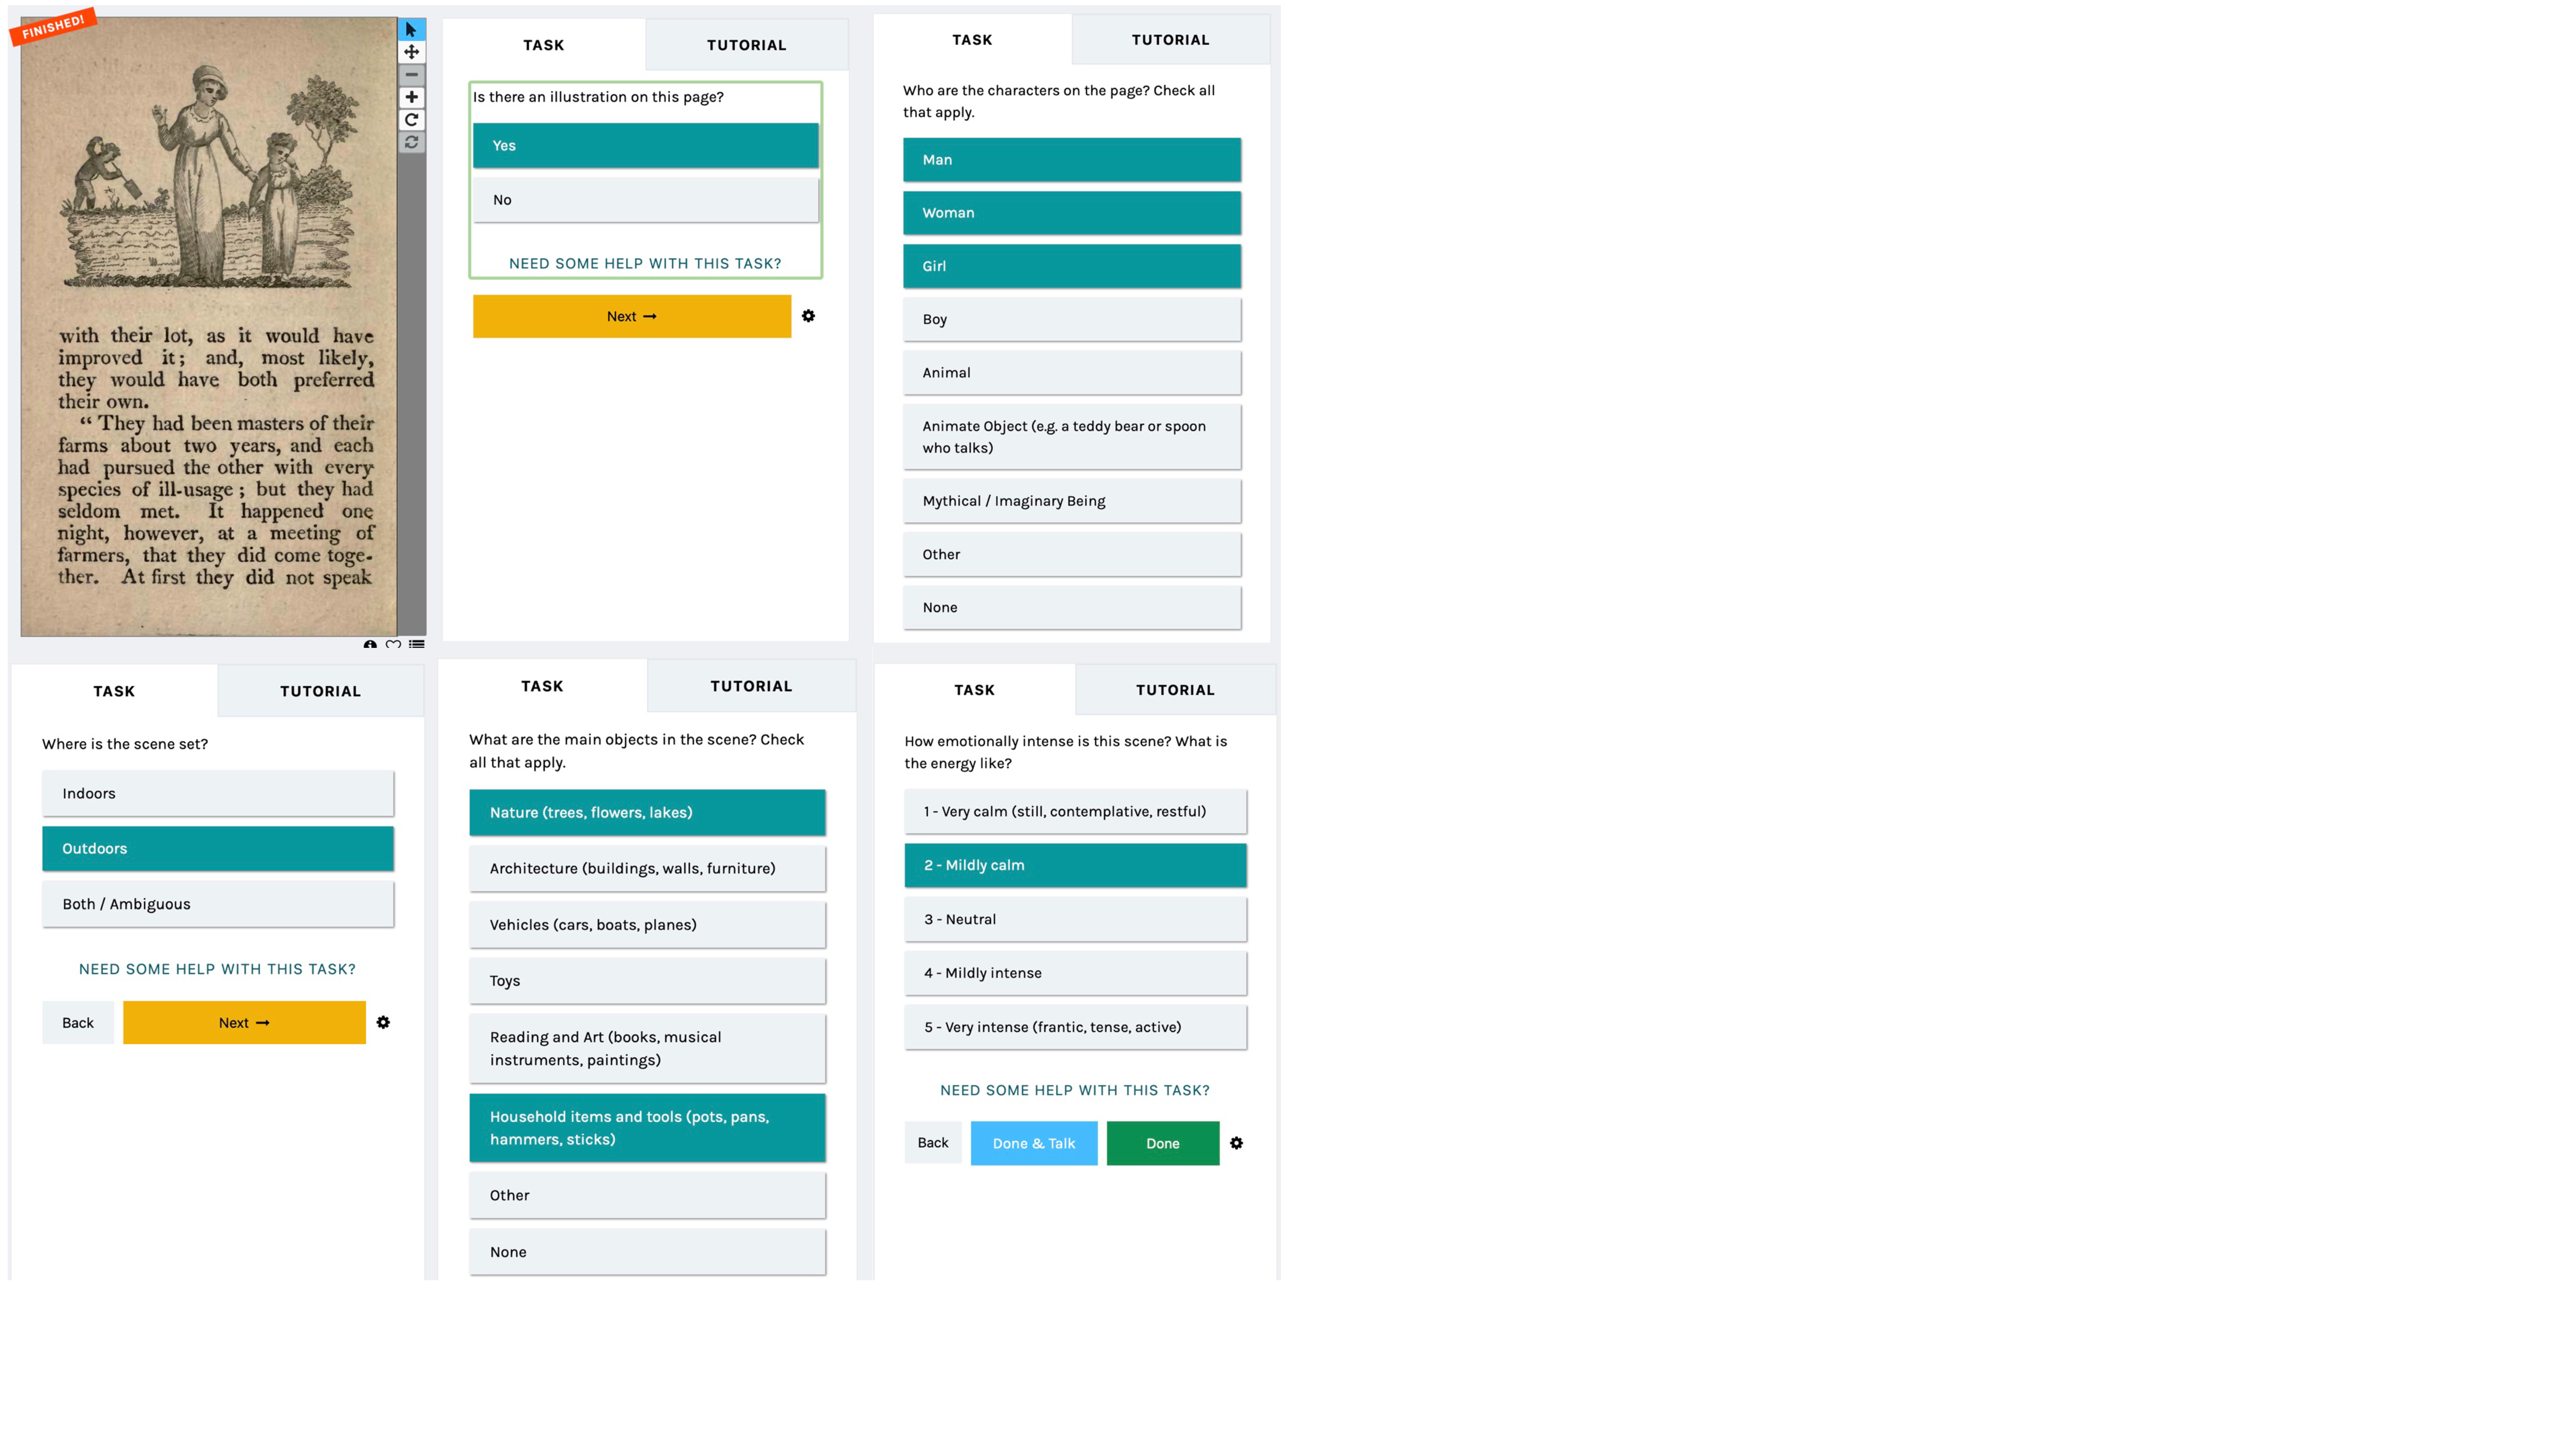
\includegraphics[width=.8\linewidth]{figures/fig_Worklow_Images.png}
  \caption{Screenshots of annotation workflow moving left to right beginning in the upper-left.}
  \label{fig:task_workflow}
\end{figure}  



\end{document}
